\Opensolutionfile{ans}[ans/ansTL-0H3-4]
\setcounter{ex}{0}
\subsubsection{Đề số 2}

\begin{ex}%[Tran Tony]%[0H2B1]
	Trong mặt phẳng tọa độ $Oxy,$ lấy điểm $M$ trên nửa đường tròn đơn vị sao cho $\widehat{xOM}=135^\circ$. Tìm hoành độ của điểm $M$.
	\choice
	{\True $-\dfrac{\sqrt{2}}{2}$}
	{$\dfrac{\sqrt{2}}{2}$}
	{$-\dfrac{\sqrt{3}}{2}$}
	{$-\dfrac{1}{2}$}
\end{ex}

\begin{ex}%[Võ Đông Phước]%[0H2B1]
	Tính giá trị của biểu thức $P=3\sin30^\circ-5\cos60^\circ+7\cos90^\circ$.
	\choice{$P=3$}
	{$P=-5$}
	{\True $P=-1$}
	{$P=7$}
\end{ex}

\begin{ex}%[Bùi Sang Thọ]%[0H2K1]
	Biết $\cos\alpha=\dfrac{1}{3}$. Giá trị đúng của biểu thức $P=\sin^2\alpha+3\cos^2\alpha$ là
	\choice
	{$\dfrac{1}{3}$}
	{$\dfrac{10}{9}$}
	{$\dfrac{11}{9}$}
	{\True $\dfrac{4}{3}$}
\end{ex}

\begin{ex}%[Bùi Sang Thọ]%[0H2K1]
	Biết $\tan\alpha=-2$. Tính giá trị của biểu thức $B=\dfrac{2+\sin\alpha}{\cos\alpha-3\sin\alpha}$.
	\choice
	{\True $-\dfrac{3}{7}$}
	{$-\dfrac{7}{3}$}
	{$\dfrac{2}{9}$}
	{$-\dfrac{2}{9}$}
\end{ex}

\begin{ex}%[0H2B1]
	Tính giá trị biểu thức $P=\cos 0^\circ + \cos 20^\circ+ \cos 40^\circ + \cdots + \cos 160^\circ + \cos 180^\circ$.
	\choice{\True $P=0$}
	{$P=-1$}
	{$P=1$}
	{$P=2$}
\end{ex}

\begin{ex}%[0H2Y3-1]
	Tam giác $ ABC$ có $ AB=\sqrt{2}$, $AC=\sqrt{3}$ và $ \widehat{C}=45^\circ $. Tính độ dài cạnh $ BC$.
	\choice
	{$ BC=\sqrt{5}$}
	{\True $ BC=\dfrac{\sqrt{6}+\sqrt{2}}{2}$}
	{$ BC=\sqrt{6}$}
	{$ BC=\dfrac{\sqrt{6}-\sqrt{2}}{2}$}
	\loigiai
	{Theo định lí hàm cô-sin, ta có\\
		$ AB^2=AC^2+BC^2-2\cdot AC\cdot BC\cdot \cos \widehat{C}\Rightarrow {(\sqrt{2} )}^2={(\sqrt{3} )}^2+BC^2-2\cdot \sqrt{3}\cdot BC\cdot \cos 45^\circ $ \\
		$ \Rightarrow BC=\dfrac{\sqrt{6}+\sqrt{2}}{2}$.}
\end{ex}

\begin{ex}%[0H2B3-1]
	Tam giác $ ABC$ có $ AB=4$, $BC=6$, $AC=2\sqrt{7}$. Điểm $ M$ thuộc đoạn $ BC$ sao cho $ MC=2MB$. Tính độ dài cạnh $ AM$.
	\choice
	{$ AM=4\sqrt{2}$}
	{$ AM=3\sqrt{2}$}
	{\True $ AM=2\sqrt{3}$}
	{$ AM=3$}
	\loigiai{
		\immini
		{
			Theo định lí hàm cô-sin, ta có\\
			$ \cos B=\dfrac{AB^2+BC^2-AC^2}{2\cdot AB\cdot BC}=\dfrac{4^2+6^2-(2\sqrt{7} )^2}{2\cdot 4\cdot 6}=\dfrac{1}{2}$.\\
			Do $ MC=2MB\Rightarrow BM=\dfrac{1}{3}BC=2$.\\
			Theo định lí hàm cô-sin, ta có\\
			$ \begin{aligned}
				AM^2&=AB^2+BM^2-2\cdot AB\cdot BM\cdot \cos B \\
				& =4^2+2^2-2\cdot 4\cdot 2\cdot \dfrac{1}{2}=12.
			\end{aligned}\\
			\Rightarrow AM=2\sqrt{3}$.
		}
		{
			\begin{tikzpicture}[scale=0.9, font=\footnotesize, line join = round, line cap = round,>=stealth]
				\tkzDefPoints{-2/0/B,0/3/A,5/0/C}
				\coordinate (M) at ($(B)!0. 33!(C)$);
				\tkzDrawPoints[fill=black](A,B,C,M)
				\tkzDrawPolygon(A,B,C)
				\tkzDrawSegments(M,A)
				\tkzLabelPoints[above](A)
				\tkzLabelPoints[below](M,B,C)
			\end{tikzpicture}
	}}
\end{ex}
\begin{ex}%[0H2B3-1]
	Cho hình thoi $ ABCD$ cạnh bằng $ 1$ cm và có $ \widehat{BAD}=60^\circ $. Tính độ dài cạnh $ AC$.
	\choice
	{$ AC=2$}
	{\True $ AC=\sqrt{3}$}
	{$ AC=2\sqrt{3}$}
	{$ AC=\sqrt{2}$}
	\loigiai{
		\immini{
			Do $ ABCD$ là hình thoi, có $ \widehat{BAD}=60^\circ \Rightarrow \widehat{ABC}=120^\circ $.\\
			Theo định lí hàm cô-sin, ta có\\
			$ \begin{aligned}
				AC^2&=AB^2+BC^2-2\cdot AB\cdot BC\cdot \cos \widehat{ABC} \\
				& =1^2+1^2-2\cdot 1\cdot 1\cdot \cos 120^\circ\\
				& =3.\\
				\Rightarrow AC=\sqrt{3}\cdot \\
			\end{aligned}$}
		{
			\begin{tikzpicture}[scale=1, font=\footnotesize, line join = round, line cap = round,>=stealth]
				\tkzDefPoints{-2/0/A,0/3/B}
				\tkzDefPointBy[rotation = center A angle -60](B) \tkzGetPoint{D}
				\coordinate (C) at ($(B)+(D)-(A)$);
				\tkzDrawPoints[fill=black](A,B,C,D)
				\tkzDrawPolygon(A,B,C,D)
				\tkzDrawSegments(C,A D,B)
				\tkzLabelPoints[above](B,C)
				\tkzLabelPoints[below](A,D)
				\tkzMarkAngles[size=0.5cm,arc=l](D,A,B)
		\end{tikzpicture}}
	}
\end{ex}

\begin{ex}%[Phạm Tuấn]%[0H2B3-1]
	Cho tam giác $ABC$ có góc $\widehat{A}=60^{\circ}$, $\widehat{B}=45^{\circ}$, $AB=25$. Độ dài cạnh $BC$ gần với giá trị nào nhất dưới đây?
	\choice
	{$22$}
	{\True $22{,}5$}
	{$24{,}5$}
	{$21{,}5$}
	\loigiai{
		Ta có $\widehat{C}=180^\circ - \widehat{A}-\widehat{B} =  180^\circ - 60^{\circ}-45^{\circ} = 75^{\circ}$. \\
		Áp dụng định lí sin ta có 
		\[ \dfrac{BC}{\sin A}=\dfrac{AB}{\sin C} \Rightarrow BC=\dfrac{AB\cdot\sin A}{\sin C}=\dfrac{25\cdot \sin 60^\circ}{\sin 75^\circ} \approx 22{,}4.\]
	}
\end{ex}

\begin{ex}%[Phạm Tuấn]%[0H2B3-1]
	Cho tam giác $ABC$ có $AB=8$, $AC = 11$, $\widehat{A}=30^\circ$.  Số đo góc $B$ gần với giá trị nào nhất dưới đây?
	\choice
	{$50{,}5^\circ$}
	{$45{,}8^\circ$}
	{$65{,}3^\circ$}
	{\True $55{,}2^\circ$}
	\loigiai{
		Áp dụng định lí côsin ta có 
		\[ BC^2=AB^2+AC^2-2AB \cdot AC \cos A =8^2+11^2-2 \cdot 8 \cdot 11 \cos 30^\circ \Rightarrow BC \approx 6{,}7.\]
		Áp dụng định lí sin ta có 
		\begin{align*}
			\dfrac{AC}{\sin B} = \dfrac{BC}{\sin A} \Rightarrow \sin B = \dfrac{AC\sin A}{BC}  = \dfrac{11 \sin 30^{\circ}}{6{,}7} \Rightarrow \widehat{B} \approx 55{,}2^\circ.  
		\end{align*}
	}
\end{ex}

\begin{ex}%[0H2B3]
	Cho tam giác $ABC$ có $BC=4$, $CA=6$, $AB=8$ và $M$ là trung điểm $BC$. Tính độ dài $AM$.
	\choice{\True $AM=\sqrt{46}$}
	{$AM=4\sqrt{6}$}
	{$AM=\sqrt{42}$}
	{$AM=\sqrt{34}$}
\end{ex}

\begin{ex}%[0H2B3]
	Cho tam giác $ABC$ có $BC=2$ , $\widehat{A}=60^\circ$. Tính bán kính $R$ của đường tròn ngoại tiếp tam giác $ABC$.
	\choice{$R=\dfrac{4\sqrt{3}}{3}$}
	{\True $R=\dfrac{2\sqrt{3}}{3}$}
	{$R=4$}
	{$R=2$}
\end{ex}

\begin{ex}%[0H2B3]
	Cho tam giác $ABC$ cân tại $A$ có diện tích $S=2\sqrt{3}$ và $BC=2\sqrt{6}$. Tính độ dài cạnh $AB$.
	\choice{\True $AB=2\sqrt{2}$}
	{$AB=2$}
	{$AB=2\sqrt{3}$}
	{$AB=4$}
\end{ex}

\begin{ex}%[0H2B3]
	Cho tam giác $ABC$ có $BC^2>AB^2+BC^2$. Mệnh đề nào sau đây là đúng?
	\choice{\True $\widehat{A}$ là góc tù}
	{$\widehat{A}$ là góc nhọn}
	{$\widehat{A}$ là góc vuông}
	{$\widehat{A}$ là góc nhỏ nhất}
\end{ex}

	\begin{ex}%[0H2Y3-1]
	Cho tam giác $ABC$ có $AB=4$, $AC=3$, $\widehat{BAC}=30^\circ$. Khi đó diện tích tam giác $ABC$ bằng
	\choice
	{\True $3$}
	{$4\sqrt{3}$}
	{$6\sqrt{3}$}
	{$6$}
	\loigiai{
		Ta có $S_{ABC}=\dfrac{1}{2}AB\cdot AC\cdot\sin\widehat{BAC}=\dfrac{4\cdot 3\cdot\sin30^\circ}{2}=3$.
	}
\end{ex}
\begin{ex}%[0H2B3-1]
	Tìm chu vi tam giác $ABC$, biết $AB=6$ và $2\sin A=3\sin B=4\sin C$.
	\choice
	{\True $26$}
	{$13$}
	{$5\sqrt{26}$}
	{$10\sqrt{6}$}
	\loigiai{
		Từ $2\sin A=3\sin B=4\sin C$ suy ra $2BC=3AC=4AB$.\\
		Mà $AB=6$ nên $AC=8$, $BC=12$. Chu vi tam giác bằng $26$.
	}
\end{ex}
\begin{ex}%[0H2B3-1]
	Cho tam giác $ABC$ có $a=13$ m, $b= 14$ m, $c=15$ m. Tính diện tích $S$ của tam giác $ABC$.
	\choice
	{\True $S= 84$ m$^2$}
	{$S= 90$ m$^2$}
	{$S= 76$ m$^2$}
	{$S= 80$ m$^2$}
	\loigiai{
		Ta có $p=\dfrac{a+b+c}{2} =21$ và $S=\sqrt{p(p-a)(p-b)(p-c)}=\sqrt{21(21-13)(21-14)(21-15)} =84$ m$^2$.	
	}
\end{ex}

\begin{ex}%[0H2B3-1]
	Tam giác $ ABC$ có $ AB=3$, $AC=6$, $\widehat{BAC}=60^\circ $. Tính độ dài đường cao $ h_a$ của tam giác.
	\choice
	{$ h_a=3\sqrt{3}$}
	{$ h_a=\sqrt{3}$}
	{$ h_a=\dfrac{3}{2}$}
	{\True $ h_a=3$}
	\loigiai
	{Áp dụng định lý hàm số cô-sin, ta có
		$ BC^2=AB^2+AC^2-2AB\cdot AC\cos A=27\Rightarrow BC=3\sqrt{3}$.\\
		Ta có $ S_{\Delta ABC}=\dfrac{1}{2}\cdot AB\cdot AC\cdot \sin{A}=\dfrac{1}{2}\cdot 3\cdot 6\cdot \sin 60^\circ=\dfrac{9\sqrt{3}}{2}$.\\
		Lại có $ S_{\Delta ABC}=\dfrac{1}{2}\cdot BC\cdot h_a\Rightarrow h_a=\dfrac{2S}{BC}=3$.}
\end{ex}

\begin{ex}%[0H2G3]
	Cho tam giác $ABC$ có chu vi bằng $6$. Tìm giá trị lớn nhất $S$ của diện tích tam giác $ABC$.
	\choice{$S=\dfrac{3\sqrt{3}}{4}$}
	{\True $S=\sqrt{3}$}
	{$S=\dfrac{2\sqrt{3}}{3}$}
	{$S=2\sqrt{3}$}
	\loigiai{
		Gọi $s$, $p$ lần lượt là diện tích và nửa chu vi của tam giác $ABC$. Theo giả thiết ta có $p=\dfrac{BC+CA+AB}{2}=3$. Ta có
		$$s=\sqrt{p(p-BC)(p-CA)(p-AB)}\le \sqrt{p\left(\dfrac{p-BC+p-CA+p-AB}{3}\right)^3}=\dfrac{p^2}{3\sqrt{3}}=\sqrt{3}.$$
		Dấu bằng xảy ra khi tam giác $ABC$ là tam giác đều. Vậy $S=\sqrt{3}$.
	}
\end{ex}

\begin{ex}%[0H2K3]
	\immini[thm]{
		Một con thuyền từ điểm $A$ ở bờ bên này sông di chuyển sang bờ sông bên kia với vận tốc $2\ \mathrm{km/h}$. Do tác động của dòng nước nên đường đi của con thuyền tạo với bờ sông một góc $70^\circ$. Biết thuyền đi từ $A$ đến $B$ mất $5$ phút và coi hai bờ sông là hai đường thẳng song song, tính độ rộng của con sông (làm tròn đến hàng đơn vị).
		\choice{$134\ \mathrm{m}$}
		{\True $157\ \mathrm{m}$}
		{$168\ \mathrm{m}$}
		{$142\ \mathrm{m}$}
	}
	{
		\begin{tikzpicture}
		\tkzDefPoints{0/0/A, -2/0/X, 4/0/Y}
		\tkzLabelPoint[below](A){$A$}
		\tkzDrawSegment(X,Y)
		\tkzDefShiftPoint[A](70:3.193){B}
		\tkzLabelPoint[above](B){$B$}
		\tkzDefPoints{-2/3/C, 4/3/D}
		\tkzDrawSegments(C,D A,B)
		\tkzMarkAngle[size=0.4](Y,A,B)
		\tkzLabelAngle[pos=0.8](Y,A,B){$70^\circ$}
		\end{tikzpicture}
	}
	\loigiai{
		Gọi $H$ là hình chiếu của $B$ trên bờ sông chứa điểm xuất phát $A$. Khi đó độ rộng của con sông là
		$$BH=BA\sin 70^\circ=2\cdot \dfrac{5}{60}\sin 70^\circ \approx 157\ (\mathrm{m}).$$
	}
\end{ex}

\begin{ex}%[Phan Văn Thành]%[0H2K3]\newline
	\immini[thm] {Một người đứng tại vị trí $E$, có chiều cao $EF = 1,8\textrm{\,m}$, quan sát một cái cây $AD$, góc nhìn $\widehat{AFG} = 45^{\circ}$. Khoảng cách từ người tới vị trí cái cây là $ED = 20\textrm{\,m}$. Tính chiều cao $AD$ của cái cây (Hình vẽ bên).
		\choice
		{\True $AD = 21,8 \textrm{\,m}$}
		{$AD = 20 \textrm{\,m}$}
		{$AD = 18,2 \textrm{\,m}$}
		{$AD = 30 \textrm{\,m}$}}{\begin{tikzpicture}[scale = 0.7, line cap=round,line join=round,>=triangle 45,x=1.0cm,y=1.0cm]
			\clip(-2.56,-1.6) rectangle (3.96,4.58);
			\fill[color=black,fill=black,fill opacity=0.1] (3,4) -- (3.56,3.98) -- (3.56,-1) -- (3,-1) -- cycle;
			\draw [color=black] (3,4)-- (3.56,3.98);
			\draw [color=black] (3.56,3.98)-- (3.56,-1);
			\draw [color=black] (3.56,-1)-- (3,-1);
			\draw [color=black] (3,-1)-- (3,4);
			\draw (-2,0)-- (-2,-1);
			\draw (-2,-1)-- (3,-1);
			\draw (-2,0)-- (3,0);
			\draw (-2,0)-- (3,4);
			\fill [color=black] (3,4) circle (1.5pt);
			\draw[color=black] (3,4.3) node {$A$};
			\fill [color=black] (3,-1) circle (1.5pt);
			\draw[color=black] (2.7,-0.7) node {$D$};
			\fill [color=black] (-2,-1) circle (1.5pt);
			\draw[color=black] (-2.3,-0.8) node {$E$};
			\fill [color=black] (-2,0) circle (1.5pt);
			\draw[color=black] (-2.2,0.3) node {$F$};
			\fill [color=black] (3,0) circle (1.5pt);
			\draw[color=black] (2.6,0.3) node {$G$};
	\end{tikzpicture}}
\end{ex}

\begin{ex}%[Phan Văn Thành]%[0H2K3]
	\immini[thm]{ Một máy bay trực thăng $A$ quan sát hai tàu $B$ và $C$. Biết trực thăng $A$ cách tàu $B$ và tàu $C$ lần lượt là  $23,8$ km và $31,9$ km. Góc nhìn từ trực thăng đến hai tàu là $83,6^\circ$. Hỏi hai tàu cách nhau một khoảng gần nhất với giá trị nào sau đây?
		\choice
		{$41,87$ km}
		{$40,87$ km}
		{\True $37,61$ km}
		{$39,61$ km}}
	{\begin{tikzpicture}
			%% Tàu a
			\def\taua[#1](#2){
				\begin{scope}[#1]
					\coordinate(a) at ($(#2)$);
					\fill[orange!40!red] ($(#2)+(0.8,0.15)$) rectangle ($(#2)+(0.9,0.25)$) ($(#2)+(1.3,0.15)$) rectangle ($(#2)+(1.4,0.25)$) ; 
					\fill[black] ($(#2)+(0.8,0.25)$) rectangle ($(#2)+(0.9,0.3)$) ($(#2)+(1.3,0.25)$) rectangle ($(#2)+(1.4,0.3)$) ; 
					\fill[cyan!80!blue] ($(#2)+(0.5,0)$) rectangle ($(#2)+(2,-0.2)$)
					($(#2)+(0.6,0.15)$) -- ($(#2)+(0.6,0)$) -- ($(#2)+(1.8,0)$) -- ($(#2)+(1.7,0.15)$) -- ($(#2)+(0.8,0.15)$);
					\foreach \a in {0.1,0.2, ...,1 }
					\fill[white] ($(#2)+(0.6+\a,0.06)$) circle (1pt) ;
					\fill (#2)--($(#2)+(-50:0.4)$)coordinate(a1)--($(a1)+(0:2)$)coordinate(a2)--($(a2)+(90:0.25)$)coordinate(a3) -- ($(a3)+(180:1.6)$)  -- (a) ;        
					\fill[red] ($(a1)!0.1cm!(a)$)coordinate(a7) -- (a1) -- (a2) -- ($(a2)!0.1cm!(a3)$) -- (a7) ; 
			\end{scope} }
			%% Tàu b
			\def\taub[#1](#2){
				\begin{scope}[#1]
					\coordinate (b) at ($(#2)$) ;
					\filldraw[black] 
					($(b)+(0:0.3)$)coordinate(c1) -- ($(c1)+(40:0.3)$)coordinate(c2) -- ($(c2)+(0:0.6)$)coordinate(c3) -- ($(c3)+(-90:0.3)$) -- (c1);
					\filldraw[white] ($(b)+(0.4,0.04)$)coordinate(d1) -- ($(b)+(0.53,0.15)$)coordinate(d2) -- ($(b)+(0.75,0.15)$) -- ($(b)+(0.75,0.04)$) -- (d1) ($(b)+(0.8,0.04)$) rectangle ($(b)+(1.1,0.15)$);
					\filldraw[gray!30!black, rounded corners=0.05cm] ($(b)+(1.65,-0.2)$) rectangle ($(b)+(1.85,0.08)$) ;
					\filldraw[red] ($(b)+(1.67,0.04)$) rectangle ($(b)+(1.83,0.05)$) ;
					\filldraw[blue!50!black] (b) to [bend right =20]  ($(b)+(-50:0.4)$)coordinate(b1) -- ($(b1)+(0:1.5)$)coordinate(b2) to [bend right=30] ($(b2)+(90:0.3)$)coordinate(b3) -- (b) ;
					\fill [black, draw=white, line width=0.15pt] ($(b)+(0.2,-0.1)$) circle (1pt);
			\end{scope} }
			%% Trực thăng
			\def\tauc[#1](#2){
				\begin{scope}[#1]
					\coordinate(c) at ($(#2)$) ;
					\shade[shading=radial, gray ] ($(c)+(0.58,0.05)$) circle (0.15cm);
					\shade[draw=gray!10, shading=radial, gray ,yscale=0.1] ($(c)+(-0.35,1)$) circle (0.6cm);
					\draw [black, line width=0.5pt] ($(c)+(-0.4,-0.4)$) -- ($(c)+(-0.85,-0.4)$)   
					($(c)+(-0.4,-0.4)$) to [bend right=30] ($(c)+(-0.35,-0.38)$)    
					($(c)+(-0.85,-0.4)$) to [bend left=30] ($(c)+(-0.9,-0.38)$) 
					($(c)+(-0.5,-0.4)$) --($(c)+(-0.5,-0.34)$) 
					($(c)+(-0.73,-0.4)$) -- ($(c)+(-0.73,-0.34)$)   ;
					\shade[ top color=gray!40!black, bottom color=gray!80!black] (c) -- ($(c)+(0.5,0)$)coordinate(e1) -- ($(c)+(0.6,0.1)$) -- ($(c)+(0.6,-0.08)$) -- ($(c)+(-0.1,-0.1)$) -- (c)  ;
					\shade[top color=gray, rounded corners,opacity=0.2] (c) -- ($(c)+(-0.3,-0.34)$) -- ($(c)+(-1,-0.34)$) -- ($(c)+(-0.7,0)$) -- (c);
					\shade[ top color=gray!30!black, bottom color=gray, rounded corners] (c) -- ($(c)+(-0.3,-0.34)$) -- ($(c)+(-1,-0.34)$) -- ($(c)+(-0.7,0)$) -- (c);
					\shade[ball color=gray] ($(c)+(-0.2,0)$) to [bend right=30] ($(c)+(-0.5,0)$) -- ($(c)+(-0.2,0)$);
					\shade[bottom color = cyan!30, top color=white, draw=black,rounded corners=0.05cm] ($(c)+ (-0.6,-0.1)$)  -- ($(c)+(-0.6,-0.25)$) -- ($(c)+(-0.8,-0.25)$) -- ($(c)+(-0.7,-0.1)$) -- ($(c)+ (-0.6,-0.1)$);
					\shade[line width=0.2pt, bottom color = cyan!30, top color=white, draw=black] ($(c)+ (-0.5,-0.1)$)  rectangle ($(c)+(-0.55,-0.15)$) 
					($(c)+ (-0.4,-0.1)$)  rectangle ($(c)+(-0.45,-0.15)$);
					\draw [black,line width=1pt, rounded corners] ($(c)+(-0.35,0.05)$) --+(0,0.067) ;
			\end{scope} }
			
			%% Code hình
			\def\b{4}
			\coordinate(B) at (0,0) ;
			\path [name path=ac1]  ($(B)+(65:\b)$)coordinate(A) --  ($(A)+(-46.4:1.5*\b)$)coordinate(C1)  ;
			\path [name path =bb] (B) -- ($(B)+(0:2*\b)$)  ;
			\path [name intersections = {of =ac1 and bb, by=C}] ;
			\draw (B)node[below]{$B$} -- (A)node[above left]{ $A$}node[midway,sloped, above]{\footnotesize $23,8\,km$} -- (C)node[below]{$C$}node[midway,sloped, above]{\footnotesize $31,9\,km$} ; 
			\draw [dashed] (B) -- (C)node[midway, above ]{\footnotesize $?\,km$} ;
			
			\fill[red!20, draw=black] (A) -- ($(A)!0.5cm!(B)$) to [bend right= 30] ($(A)!0.5cm!(C)$) -- (A)node[shift={(-77:.8)}]{ \footnotesize \textcolor{black}{ $83,6^\circ$}} ;
			\fill[black] (A) circle (1.5pt) (B) circle (1.5pt) (C) circle (1.5pt) ;
			\draw ($(B)+(-2,0.2)$)coordinate(B1)   ($(C)+(0.2,0.2)$)coordinate(C1) 
			($(A)+(0.8,0.5)$)coordinate(A1)      
			;
			\taua[scale=0.8](B1)
			\taub[scale=0.8](C1)
			\tauc[scale=1](A1)
	\end{tikzpicture}}
\end{ex}

\begin{ex}%[Phan Văn Thành]%[0H2K3]\newline
	\immini[thm]{Hai thành phố $A$ và $B$ cách nhau một con sông. Người ta xây dựng một cây cầu $EF = 1\textrm{\,km}$ bắc qua sông biết rằng thành phố $A$ cách con sông một khoảng là $4\textrm{\,km}$ và thành phố $B$ cách con sông một khoảng là $8\textrm{\,km}$ (hình vẽ), $HE = 3 \textrm{\,km}$, $KF = 6 \textrm{\,km}$. Tính tổng quãng đường $d$ đi từ $A$ đến $B$ (đi theo đường $AEFB$).
		\choice
		{\True $d = 16\textrm{\,km}$}
		{$d = 15\textrm{\,km}$}
		{$d = 22\textrm{\,km}$}
		{$d = 21\textrm{\,km}$}}
	{\begin{tikzpicture}[scale = 0.7, line cap=round,line join=round,>=triangle 45,x=1.0cm,y=1.0cm]
			\clip(-0.86,-1.64) rectangle (9.66,5.28);
			\draw (3,5)-- (3,-1);
			\draw (5,5)-- (5,-1);
			\draw (0,4)-- (3,4);
			\draw (3,2)-- (5,2);
			\draw (5,0)-- (9,0);
			\draw (0,4)-- (3,2);
			\draw (5,2)-- (9,0);
			\draw (1,4.7) node[anchor=north west] {\scriptsize 4km};
			\draw (6.36,-0.12) node[anchor=north west] {\scriptsize 8km};
			\fill [color=black] (0,4) circle (1.5pt);
			\draw[color=black] (-0.38,4.08) node {$A$};
			\fill [color=black] (3,4) circle (1.5pt);
			\draw[color=black] (2.78,4.28) node {$H$};
			\fill [color=black] (3,2) circle (1.5pt);
			\draw[color=black] (2.6,1.8) node {$E$};
			\fill [color=black] (5,2) circle (1.5pt);
			\draw[color=black] (5.2,2.3) node {$F$};
			\fill [color=black] (9,0) circle (1.5pt);
			\draw[color=black] (9.32,0.16) node {$B$};
			\fill [color=black] (5,0) circle (1.5pt);
			\draw[color=black] (5.22,-0.4) node {$K$};
	\end{tikzpicture}}
\end{ex}

\begin{ex}
	\immini[thm]{Một người đứng cách thân một cái quạt gió $16 \mathrm{~m}$ và nhìn thấy tâm của cánh quạt với góc nâng $56,5^{\circ}$ (Hình vẽ bên). Tính khoảng cách từ tâm của cánh quạt đến mặt đất. Cho biết khoảng cách từ mắt của người đó đến mặt đất là 1,5 m.
	\haicot
	{20,8 m }
	{35,2 m }
	{28,5 m }
	{\True 25,7 m}}{
	\begin{tikzpicture}[smooth,font=\footnotesize,scale=1]
		\coordinate (M) at ($(4,4.16)+(-60:2cm)$);
		\coordinate (N) at ($(4,4.16)+(60:2cm)$);
		\coordinate (K) at ($(4,4.16)+(180:2cm)$);
		\fill[color=red](-0.05,1)--(0.05,1)--(0.05,0)--(-0.05,0)--cycle;
		\fill[color=blue](3.95,0)--(4.05,0)--(4.05,4)--(3.95,4)--cycle;
		\fill[ball color=red](0,1.16) circle (0.16);
		\fill[ball color=blue](4,4.16) circle (0.16);
		\draw[dashed,blue] (0.16,1.16)--(3.95,1.16) (0.16,1.16)--(3.84,4.16);
		\draw[very thick,blue] (4,4.16)--(M) (4,4.16)--(N) (4,4.16)--(K);
		\path
		(3.95,1.16)--(3.95,0) node[below,midway,sloped,scale=1]{$1.5$m }
		(0.16,1.16)--(3.95,1.16) node[below,midway,sloped,scale=1]{$16$m };
		\node[below] at (0,-0.2) {Người};
		\node[below] at (4,-0.2) {Quạt gió};
		\node[right] at (0.9,1.45) {$56,5^\circ$};
		\begin{scope}
			\clip (3.95,1.16)--(0.16,1.16)--(3.84,4.16);
			\draw[double] (0.16,1.16) circle(0.7cm);
		\end{scope}
	
\end{tikzpicture}}
	\loigiai{
	\immini{Vì tam giác $A B C$ vuông tại $C$ nên ta có $$\tan A=\dfrac{B C}{A C}=\dfrac{B C}{16}\Rightarrow \mathrm{BC}=16 \cdot \tan \mathrm{A}=16 \cdot \tan 56,5^{\circ} \approx 24,2 \mathrm{~m}$$
	Do đó $BD=BC+CD=24,2+1,5=25,7 \mathrm{~m}$.\\
	Vậy khoảng cách từ tâm của cánh quạt đến mặt đất khoảng 25,7 m.}{
		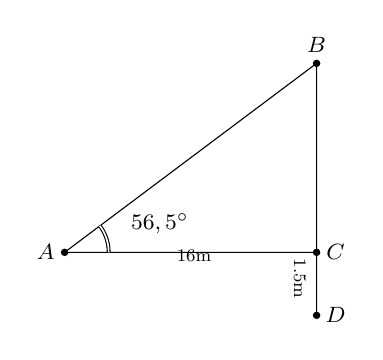
\begin{tikzpicture}[smooth,font=\footnotesize,scale=0.8]
		\path
		(0,1) coordinate (A)
		(4,4) coordinate (B)
		(4,1) coordinate (C)
		(4,0) coordinate (D);
		\draw (A)--(B)--(D) (A)--(C);
		\foreach \x/\g in {A/180,B/90,C/0,D/0} \draw [fill=black] (\x) circle (.05) + (\g:.3) node{$\x$};
		\begin{scope}
			\clip (B)--(A)--(C);
			\draw[double] (A) circle(0.7cm);
		\end{scope}
	\node[right] at (0.9,1.45) {$56,5^\circ$};
	\path
	(3.95,1.16)--(3.95,0) node[below,midway,sloped,scale=0.8]{$1.5$m }
	(0.16,1.16)--(3.95,1.16) node[below,midway,sloped,scale=0.8]{$16$m };
\end{tikzpicture}}}
\end{ex}
\begin{ex}
	\immini[thm]{Trên bảng đồ địa lý, người ta thường gọi tứ giác với 4 đỉnh lần lượt là các thành phố Hà Tiên, Châu Đốc, Long Xuyên, Rạch Giá là tứ giác Long Xuyên. Dựa vào các khoảng cách đã cho ở hình bên, tính khoảng cách giữa Châu Đốc và Rạch Giá. 
	\haicot
	{80 km }
	{\True 75,7 km}
	{120 km }
	{70 km }}{
		\begin{tikzpicture}[smooth,font=\footnotesize,scale=1]
		\path
		(0,0) coordinate (H)
		(5,0) coordinate (L)
		(3.2,1.7) coordinate (C)
		(3,-2) coordinate (R);
		\draw[thick] (H)--(C)--(L)--(R)--(H)--(L);
		\draw[dashed,blue] (R)--(C);
		\foreach \x/\g in {H/180,L/0,C/90,R/-90} \draw [fill=magenta] (\x) circle (.1) + (\g:.3) node{$\x$};
		\path (H)--(C) node[above,midway,sloped,scale=.8]{$78$ km }
		(L)--(C) node[above,midway,sloped,scale=.8]{$49$ km }
		(H)--(R) node[below,midway,sloped,scale=.7]{$77$ km }
		(R)--(L) node[below,midway,sloped,scale=.7]{$56$ km }
		(H)--(L) node[below,midway,sloped,scale=.7]{$104$ km };
		\node[below right] at (5,-0.4) {Long Xuyên};
		\node[below left] at (0,-0.4) {Hà Tiên};
		\node[below] at (3,-2.6) {Rạch Giá};
		\node[above] at (3.2,2.2) {Châu Đốc};
		\end{tikzpicture}}
	\loigiai{
		Áp dụng hệ quả của định lí côsin cho tam giác $CHL$, ta có
		
			$$\cos \widehat{CLH}=\dfrac{C L^{2}+H L^{2}-C H^{2}}{2 . C L \cdot H L}=\dfrac{49^{2}+104^{2}-78^{2}}{2.49 .104} \approx 0,6999			\Rightarrow \widehat{C L H} \approx 45^{\circ} 35^{\prime} 
			$$
		Áp dụng hệ quả của định lí côsin cho tam giác $RHL$ ta có:
		$$
		\cos \widehat{RLH}=\dfrac{RL^2+HL^2-RH^2}{2 \cdot RL \cdot H L}=\frac{56^2+104^2-77^2}{2.56 .104} \approx 0,6888 \Rightarrow \widehat{RLH} \approx 46^{\circ} 28' .
		$$
		Suy ra $\widehat{C L R}=\widehat{C L H}+\widehat{R L H} \approx 45^{\circ} 35^{\prime}+46^{\circ} 28^{\prime} \approx 92^{\circ} 3^{\prime}$.\\
		Áp dụng định lí côsin cho tam giác $LCR$, ta có
		$$
		CR^{2}=CL^{2}+LR^{2}-2 \cdot CL\cdot LR \cdot \cos\widehat{CLR}\Rightarrow CR\approx 75,7$$
		Vậy khoảng cách giữa Châu Đốc và Rạch Giá khoảng 75,7 km.}
\end{ex}




\centerline{\textbf{---HẾT---}}
\Closesolutionfile{ans}
